Our ultimate aim is to use Theorem~\ref{the:criterion} to certify the faithfulness of $\Psi_4$ up to some large number of intersections between the pairs of arcs appearing in the theorem. Given that the existence of a pair $(\alpha, \beta)$ with $\beta$ of type $(3,4)$ and zero Burau polynomial is equivalent to the existence of some pair $(\alpha', \beta')$ with $\beta '$ of type $(0,3)$ and zero Burau polynomial, we limit our search to those of the former type. Thus we will show that, up to some large bound $N$, any arcs $\alpha$ of type $(1,2)$ and $\beta$ of type $(3,4)$ intersecting $N$ times or fewer have non-zero Burau polynomial.
 
In practice, the techniques we use could be implemented to approach pairs of the latter type. Bigelow carried out a computer search on this latter type using different methods \cite{Big02}. There, his `noodles' and `forks' are equivalent to arc-pairs of types $(1,2)$ and $(0,3)$: the fork's tine is an arc of type $(1,2)$, while a noodle $N$ gives rise to an arc of type $(0,i)$, by joining $p_0$ to the puncture $p_i$ separated from the rest by $N$. We note that passing from a noodle to its arc halves the intersection number with the fork's tine, resulting in the halving from 2000 to 1000 stated in this paper's introduction.

Since our focus will be on arc pairs $(\alpha, \beta)$ of types $(1,2)$ and $(3,4)$, we will call any such pair a \emph{Burau pair}.
 
\subsection{Train tracks}

Given an arc in $D_n$, we encode its path using a finite data set, via a train track. For our purposes, a \emph{train track} $\tau$ in the punctured disk $D_n$ is an embedded trivalent graph $\Gamma$, where all edges incident at a vertex $v$ have a well-defined, common tangent line at $v$. It is also required that each $v$ has exactly two edges entering from one direction. We refer to the edges of $\Gamma$ as \emph{rails} and the vertices as \emph{switches}. Figure~\ref{track} displays an example of a train track in $D_4$. We note that our definition is weaker than the usual definition of train track, in that the complement of a train track may have a disk as a connected component.

Let $\tau$ be some train track in $D_n$. A simple closed curve $\gamma$ in $D_n$ is \emph{carried by $\tau$} if $\gamma$ is homotopic to a regular smooth path in $\tau$. The number of points in $\gamma$ that are homotoped to the same point of a rail $r$ is well-defined over all such homotopies, called the \emph{weight} of $\gamma$ on $r$. More loosely, the weight of $\gamma$ on $r$ is the number of segments near $r$ after $\gamma$ has been homotoped close to $\tau$.

Given a switch $v$, let $w_1$, $w_2$ and $w_3$ denote the weights of a curve $\gamma$, carried by $\tau$, on the rails $r_1$, $r_2$ and $r_3$ of $v$, respectively. If $r_1$ and $r_2$ approach $v$ from the same direction, the \emph{switch condition}
\[w_1+w_2 = w_3 \]
must hold between the weights. Any set of weights on the rails of $\Gamma$ that satisfies every switch condition gives rise to some simple, closed multi-curve (that is, some collection of pairwise disjoint simple closed curves).

We will be concerned with describing arcs rather than simple closed curves. To pass from the former to the latter, we take the boundary of a regular neighborhood of the arc. We discuss how to reverse this procedure in Section 4, giving necessary and sufficient conditions that a given multi-curve contains a curve that arises from an arc in this fashion. In practice, we will discard any proper multi-curve (i.e. a multi-curve with at least two components). The procedure we use is discussed at the end of Section 4.

\subsection{A universal track}

Due to our weakened definition of a train track in $D_n$, we may carry all simple closed curves in $D_4$ on a single track. This track is seen in Figure~\ref{track}, and we denote it by $\mu$.
\begin{figure}[h]
\begin{center}
\begin{overpic}[width=2.7in]{ideal.png}
\end{overpic}
\caption{The universal train track $\mu$, together with an ideal decomposition of $D_4$ into two hexagons.}
\label{track}
\end{center}
\end{figure}
\begin{proposition}\label{pro:universal}Any simple closed curve $\gamma$ in $D_4$ is carried by the train track $\mu$.
\end{proposition} 
\begin{proof}
We decompose $D_4$ as the (ideal) polygonal complex seen in Figure~\ref{track}. Up to isotopy, any simple closed curve $\gamma$ may be described via a sequence of line segments, each of which enters then leaves some polygon in this decomposition of $D_4$. We may assume that no segment enters and leaves a polygon on the same 1-cell, and that no segment intersects a 1-cell lying on the boundary of $D_4$. Each segment, up to isotopy, is uniquely determined by which two 1-cells it meets.

To show that any $\gamma$ is carried by the track $\mu$, it thus suffices to show that the finitely many possible line segments in the decomposition's polygons all may be homotoped so that they lie on the rails of $\tau$. Figure~\ref{track} may be used to verify this.
\end{proof}

\subsection{Standard forms for arcs}
\label{subsect:standardForms}
A priori, to use Theorem~\ref{the:criterion} to investigate the faithfulness of $\Psi_4$, there are infinitely many pairs of arcs with a fixed intersection number for which to calculate the Burau polynomial. In this section, we describe how to reduce to checking only finitely many pairs for each intersection number.

Our first reduction follows from the definition of the Burau polynomial, since each intersection between $\alpha$ and $\beta$ contributes $\pm t^i$ to their polynomial.

\textbf{Reduction I:} We need only calculate the Burau polynomial of arc pairs $(\alpha, \beta)$ whose (geometric) intersection number is even and positive.

Our subsequent reductions utilize the action of the braid group $B_4$ on $D_4$. As discussed by Bigelow, any Burau pair $(\alpha ', \beta ')$ yields an explicit, non-trivial element in the kernel of $\Psi_n$. Letting $T_{\gamma}$ denote the half-twist about an arc $\gamma$ in $D_4$, this explicit element is the commutator $[T_{\alpha '}, T_{\beta '}]$. Now, observe that any arc of type $(1,2)$ may be carried to the straight line arc $\alpha$ seen in Figure~\ref{disk} by acting by an appropriate member $\sigma$ of the braid group $B_4$. It follows from Proposition~\ref{preserve} that $(\alpha ', \beta ')$ is a Burau pair if and only if $(\alpha, \sigma \cdot \beta ')$ is a Burau pair. This leads to our second reduction.

\emph{Our subsequent reductions utilize the action of the braid group $B_4$ on $D_4$. Observe that any arc of type $(1,2)$ may be carried to the straight line arc $\alpha$ seen in Figure~\ref{disk} by acting by an appropriate member $\sigma$ of the braid group $B_4$. It follows from Proposition~\ref{preserve} that $(\alpha ', \beta ')$ has the same Burau polynomial as $(\alpha, \sigma \cdot \beta ')$. This leads to our second reduction.}

\textbf{Reduction II:} We need only calculate the Burau polynomial of arc pairs $(\alpha, \beta)$ where $\alpha$ is the straight line arc joining $p_1$ and $p_2$.

To perform our final reduction, let $N$ denote a regular neighborhood of the arc $\alpha$, and let $B_4(\partial N)$ denote the stabilizer in $B_4$ of the isotopy class of the boundary $\partial N$ of $N$. By letting the marked points $p_3$ and $p_4$ wander in the twice-punctured annulus $D_4 \setminus N$, we see that any arc $\beta '$ of type $(3,4)$ has a (perhaps different) representative whose initial and terminal segments are one of the possibilities seen in Figures \ref{initial} and \ref{terminal}, respectively. This is because such a wandering may be achieved by acting by a braid in $B_4(\partial N)$. 

\begin{figure}
\centering
\begin{subfigure}[t]{0.4\textwidth}\centering
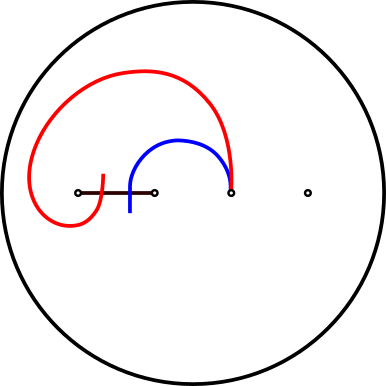
\includegraphics[width=2in]{initial.png}  
\caption{}
\label{initial}
\end{subfigure}
\quad
\begin{subfigure}[t]{0.4\textwidth}\centering
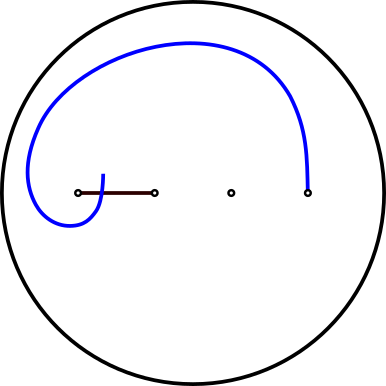
\includegraphics[width=2in]{terminal.png} 
\caption{}
\label{terminal}
\end{subfigure}
\caption{Initial (a) and terminal (b) segments of the arc $\beta$ after our reduction process. We orient $\beta$ so that it begins at $p_3$ and ends at $p_4$.} \label{segments}
\end{figure}

Suppose two arcs $\beta_1$ and $\beta_2$ have as initial and terminal segments one of the choices shown in Figure~\ref{segments}. If $\beta_1$ and $\beta_2$ lie in the same orbit under the action of $B_4(\partial N)$, then they are isotopic rel. endpoints. We see this as follows. Certainly, if $\beta_1$ and $\beta_2$ belong to the same $B_4(\partial N)$-orbit, they must have the same choice of initial and terminal segment, since $B_4(\partial N)$ acts on the annulus $D_4 \setminus N$, preserving whether the segments both intersect $\alpha$ on the same or opposing sides. Assume $\beta_1$ and $\beta_2$ agree on their initial and terminal segments and belong to the same $B_4(\partial N)$-orbit. Then any braid $\sigma \in B_4(\partial N)$ mapping $\beta_1$ to $\beta_2$ must stabilize the isotopy class of a regular neighborhood of the union of $\alpha$ together with the initial and terminal segments of $\beta_1$. Any such $\sigma$ must be a power of the Dehn twist about a curve isotopic to the boundary of $D_4$, and hence we have $\beta_1 = \beta_2$. We are thus led to make the following reduction.

\textbf{Reduction III:} We need only calculate the Burau polynomial of arc pairs $(\alpha, \beta)$ where $\beta$ has initial and terminal segments as seen in Figure \ref{segments}.

To conclude this section, we summarize our reduction process. The above discussion allows us to only consider arc pairs $(\alpha, \beta)$ that essentially intersect a positive, even number of times, such that $\alpha$ is the straight-line arc from $p_1$ to $p_2$ and $\beta$ has one of the initial and terminal segment choices displayed in Figure~\ref{segments}. No such arcs forming a pair with $\alpha$ may be carried to one another via an element of $B_4$ without changing the isotopy class of the fixed arc $\alpha$.

Note that, given our reductions, there are finitely many arcs $\beta$ that intersect $\alpha$ some fixed number of times. We remark that such an easily described set of reductions is enjoyed only by the four-punctured disk $D_4$: for larger $n$, the presence of punctures without arcs attached make the situation inside $D_n$ more challenging to report.


